\chapter{\texorpdfstring{Problemi intrattabili - Teoria $\mathbb{NP}$-completi}{Problemi intrattabili - Teoria NP-completi}}

In questo capitolo si andranno ad analizzare problemi il quale tempo di esecuzione non cresce in maniera polinomiale ($O(n^k)$ con $k\in\mathbb{N}$), dunque esistono problemi che per essere risolti richiedono un tempo almeno esponenziale ($\mathbb{EXPTIME}$), alcuni di questi possono essere la valutazione della posizione degli scacchi, il problema delle torri di \textit{Hanoi}. Inoltre esistono problemi che non hanno soluzione, come l'\textit{Halting Problem}.\newline
Tutti i problemi di questa classe hanno in comune il fatto che non è stata dimostrata né l'esistenza, né l'inesistenza di un algoritmo che possa risolverli in tempo polinomiale. Questi problemi sono stati definiti \textbf{intrattabili}.\newline
Prima di prendere in considerazione alcuni esempi, vediamo alcune definizioni:
\begin{definition}[Problema astratto]
    Un \textbf{problema astratto} è una relazione binaria $R\subseteq I\times S$ tra un insieme di istanze $I$ del problema ed un insieme di soluzioni $S$ del problema.\newline
    Esempio: \textit{shortest-path} è un problema astratto, in quanto l'istanza è un grafo $G$ e la soluzione è il cammino più breve tra due nodi $u$ e $v$ ($V,E,u,v$).
\end{definition}
Anche per questa classe di problemi possiamo distinguere diverse categorie:
\begin{definition}
    \item[Ottimizzazione] Data una istanza, trovarne la migliore tramite un criterio specifico
    \item[Ricerca] Data una istanza, trovare una soluzione tra quelle esistenti
    \item[Decisione] Data una istanza, determinare se esiste una soluzione che soddisfi un certo criterio
\end{definition}
I problemi di ottimizzazione contengono infatti i problemi di ricerca e di decisione, in quanto per risolvere un problema di ottimizzazione è necessario prima trovare una soluzione e poi determinare se questa è la migliore. Inoltre i problemi di ottimizzazione e decisione possono essere convertiti l'uno nell'altro, in quanto è possibile trasformare un problema di ottimizzazione in uno di decisione e viceversa. Ad esempio, il problema di ottimizzazione del cammino più breve può essere trasformato in un problema di decisione chiedendo se esiste un cammino di lunghezza minore di $k$.
\section{Riduzioni}
    La \textbf{riduzione polinomiale} viene definita come: presi due problemi decisionali $R_1\subseteq I_1\times\{0,1\}$ e $R_2\subseteq I_2\times\{0,1\}$, allora $R_1$ è riducibile polinomialmente a $R_2$ ($R_1\leq_p R_2$) se esiste una funzione computabile in tempo polinomiale $f:I_1\to I_2$ tale che:
    \begin{itemize}
        \item $f$ è calcolabile in tempo polinomiale
        \item per ogni istanza $x\in I_1$, e ogni soluzione $y\in S_1$ allora $(x,s)\in R_1$ se e solo se $(f(x),s)\in R_2$
    \end{itemize}
    \subsubsection{Colorazione di un grafo}
        Il problema della colorazione di un grafo è un problema di decisione o di ottimizzazione, in cui si chiede se è possibile colorare i vertici di un grafo in modo tale che nessun arco congiunga due vertici dello stesso colore. Dal punto di vista dell'ottimizzazione ci chiediamo quale sia il numero minimo di colori necessari per colorare il grafo, mentre dal punto di vista della decisione ci chiediamo se è possibile colorare il grafo con un numero $k$ di colori.\newline
        Il \textit{sudoku} anche se possa sembrare lontano da questo problema, in realtà è un problema di colorazione di un grafo. Infatti, possiamo rappresentare il \textit{sudoku} come un grafo in cui i vertici rappresentano le celle del \textit{sudoku} e gli archi rappresentano le relazioni tra le celle. In questo modo, il problema di risolvere un \textit{sudoku} diventa un problema di colorazione di un grafo, in cui dobbiamo colorare le celle in modo tale che nessuna cella adiacente abbia lo stesso colore. Per il \textit{sudoku} infatti il problema decisionale sta nel, data una matrice $n^2\times n^2$ determinare se esiste un modo per l'assegnamento di $n^2$ colori a $n^2$ celle in modo tale che nessuna cella adiacente abbia lo stesso colore. Il problema di ottimizzazione invece sta nel determinare il numero minimo di colori necessari per colorare il grafo.
    \subsubsection{Insieme Indipendente}
        Un insieme indipendente è un sottoinsieme di vertici di un grafo non orientato tale che nessun arco congiunga due vertici dello stesso insieme. Dunque: $$
            \forall(x,y)\in E: x\not\in S\land y\not\in S
        $$
        Prendendo in considerazione il seguente grafo:
        \begin{figure}
            \centering
            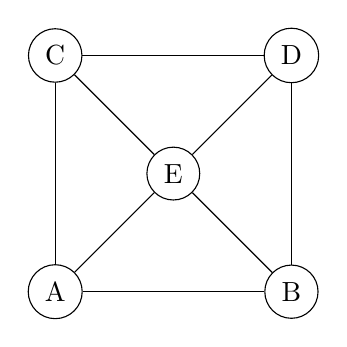
\begin{tikzpicture}
                \node[draw, circle] (a) at (0,0) {A};
                \node[draw, circle] (b) at (3,0) {B};
                \node[draw, circle] (c) at (0,3) {C};
                \node[draw, circle] (d) at (3,3) {D};
                \node[draw, circle] (e) at (1.5,1.5) {E};
                \draw (a) -- (b);
                \draw (a) -- (c);
                \draw (b) -- (d);
                \draw (c) -- (d);
                \draw (a) -- (e);
                \draw (b) -- (e);
                \draw (c) -- (e);
                \draw (d) -- (e);
            \end{tikzpicture}
            \caption{Grafo con vertici A, B, C, D, E}
        \end{figure}
        In questo grafo al massimo avremmo un insieme indipendente contenente due vertici, ad esempio $\{A,C\}$ o $\{B,D\}$. Se provassimo a prendere tre vertici, ad esempio $\{A,B,C\}$, ci accorgeremmo che esiste un arco che congiunge i vertici $A$ e $B$. 
    \subsubsection{Vertex-Cover}
        La copertura dei vertici è un sottoinsieme di vertici di un grafo non orientato tale che ogni arco del grafo ha almeno un estremo in questo insieme. Dunque: $$
            \forall(x,y)\in E: x\in S\lor y\in S
        $$
        \paragraph{Vertex-Cover, Ottimizzazione} Il problema dell'insieme indipendente è un problema di ottimizzazione, nel quale dato un grafo non orientato $G=(V,E)$, si chiede di restituire la copertura dei vertici di dimensione minima.
        \paragraph{Vertex-Cover, Decisione} Il problema dell'insieme indipendente è un problema di decisione, nel quale dato un grafo non orientato $G=(V,E)$ e un numero intero $k$, si chiede se esiste un insieme indipendente di dimensione al massimo $k$.
    \subsubsection{Riduzione per problewmi duali} 
        Nell'esempio precedente abbiamo visto che il problema dell'insieme indipendente è un problema duale del problema della copertura dei vertici. Infatti, se esiste un insieme indipendente di dimensione $k$, allora esiste una copertura dei vertici di dimensione al massimo $|V|-k$. Dunque, se $S\subseteq V$ è un \textsc{independent set} $\Rightarrow V-S$ è un \textsc{vertex cover}. Dunque possiamo dire che:
        $$
            \textsc{vertex-cover} \leq_p \textsc{independent-set}\\
            \textsc{independent-set} \leq_p \textsc{vertex-cover}
        $$
        Dunque possiamo dire che i due problemi sono duali, e quindi se uno dei due è NP-completo, anche l'altro lo è. Infatti, se esiste un algoritmo polinomiale per risolvere uno dei due problemi, allora esiste un algoritmo polinomiale per risolvere anche l'altro.
    \subsubsection{\texttt{SAT}}
        \texttt{SAT} è un problem a di formule booleane in forma normale congiunta, ovvero dato un insieme $V$ contenente $n$ variabili booleane, ed inoltre:
        \begin{itemize}
            \item un letterale, ovvero una variabile booleana o la sua negazione
            \item una clausola, ovvero una disgiunzione di letterali (separati da $\lor$)
            \item una formula in forma normale congiunta, ovvero una congiunzione di clausole (separate da $\land$)
        \end{itemize}
        Dunque, una formula booleana in forma normale congiunta è una formula booleana che può essere scritta come una congiunzione di clausole, dove ogni clausola è una disgiunzione di letterali. Ad esempio, la formula booleana $(x_1\lor x_2)\land(\neg x_1\lor x_3)$ è in forma normale congiunta, in quanto è una congiunzione di due clausole: $C_1=(x_1\lor x_2)$ e $C_2=(\neg x_1\lor x_3)$. In questo caso abbiamo tre variabili booleane: $x_1$, $x_2$ e $x_3$.\newline
        La soddisfacibilità di una formula booleana in forma normale congiunta è il problema di determinare se esiste un'assegnazione di valori booleani alle variabili in modo tale che la formula sia vera. Ad esempio, per la formula booleana $(x_1\lor x_2)\land(\neg x_1\lor x_3)$, l'assegnazione $x_1=true$, $x_2=false$ e $x_3=true$ rende la formula vera, quindi la formula è soddisfacibile.\newline
        Per risolvere questo problema si potrebbe pensare di ``provare tutte le possibilità'' il che porta ad una complessità non polinomiale, in quanto il numero di possibilità è $2^n$ (dove $n$ è il numero di variabili booleane). 
    \subsubsection{3-SAT}
        Il problema \texttt{3-SAT} è una variante del problema \texttt{SAT}, in cui ogni clausola contiene esattamente tre letterali. Dunque, una formula booleana in forma normale congiunta è in forma normale congiunta 3 se ogni clausola contiene esattamente tre letterali. Ad esempio, la formula booleana $(x_1\lor x_2\lor x_3)\land(\neg x_1\lor x_2\lor x_3)\land(x_1\lor \neg x_2\lor \neg x_3)$ è in forma normale congiunta 3, in quanto è una congiunzione di tre clausole: $C_1=(x_1\lor x_2\lor x_3)$, $C_2=(\neg x_1\lor x_2\lor x_3)$ e $C_3=(x_1\lor \neg x_2\lor \neg x_3)$.
        \paragraph{Obbiettivo} L'obbiettivo è quello di dimostrare che $3-\textsc{sat}\leq_p \textsc{Independent-set} $.
        Possiamo definire il grafo dove per ogni clausola aggiungiamo un trio di nodi collegati da un arco, e per ogni letterale aggiungiamo un arco tra i nodi che rappresentano lo rappresentano e le clausole nel quale questo letterale è presente negato. Dunque la precedente formula può essere rappresentata come:
        \begin{figure}[H]
            \centering
            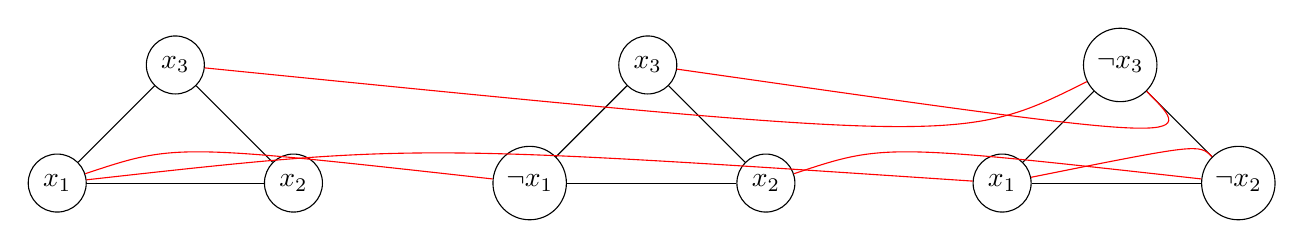
\begin{tikzpicture}
                \node[draw, circle] (x11) at (0,0) {$x_1$};
                \node[draw, circle] (x21) at (3,0) {$x_2$};
                \node[draw, circle] (x31) at (1.5,1.5) {$x_3$};
                \node[draw, circle] (x12) at (6,0) {$\neg x_1$};
                \node[draw, circle] (x22) at (9,0) {$x_2$};
                \node[draw, circle] (x32) at (7.5,1.5) {$x_3$};
                \node[draw, circle] (x13) at (12,0) {$x_1$};
                \node[draw, circle] (x23) at (15,0) {$\neg x_2$};
                \node[draw, circle] (x33) at (13.5,1.5) {$\neg x_3$};

                \draw[smooth] (x11) -- (x21);
                \draw[smooth] (x11) -- (x31);
                \draw[smooth] (x21) -- (x31);
                \draw[smooth] (x12) -- (x22);
                \draw[smooth] (x12) -- (x32);
                \draw[smooth] (x22) -- (x32);
                \draw[smooth] (x13) -- (x23);
                \draw[smooth] (x13) -- (x33);
                \draw[smooth] (x23) -- (x33);
                \draw[smooth, color=red] (x11) .. controls (1.5,0.5) and (1.5,0.5) .. (x12);
                \draw[smooth, color=red] (x11) .. controls (4.5,0.5) and (4.5,0.5) .. (x13);
                \draw[smooth, color=red] (x22) .. controls (10.5,0.5) and (10.5,0.5) .. (x23);
                \draw[smooth, color=red] (x23) .. controls (14.5,0.5) and (14.5,0.5) .. (x13);
                \draw[smooth, color=red] (x33) .. controls (14.5,0.5) and (14.5,0.5) .. (x32);
                \draw[smooth, color=red] (x33) .. controls (11.5,0.5) and (11.5,0.5) .. (x31);
                % TODO: Finire il grafo

            \end{tikzpicture}
        \end{figure}
        Dunque, se esiste un insieme indipendente di dimensione $k$ allora esiste una soluzione per il problema \texttt{3-SAT} di dimensione $k$. Quindi: $$
            3-\textsc{SAT} \leq_p \textsc{Independent-set}
        $$
        Ma è dimostrabile che per ogni $\texttt{SAT}$ esiste un $3-\texttt{SAT}$, associato, basta spezzare la clausola in $3$ parti, e aggiungere una variabile booleana che le colleghi. Dunque:
        $$
            \texttt{SAT} \leq_p 3-\texttt{SAT}
        $$
        Dunque possiamo dire che:
        $$
            \texttt{SAT} \leq_p \texttt{Independent-set}
        $$
        Dunque possiamo dire che:
        $$
            \texttt{SAT} \leq_p 3-\texttt{SAT} \leq_p \texttt{Independent-set} \leq_p \texttt{Vertex-cover}
        $$
        Dunque risolvendo uno qualsiasi di questi problemi, possiamo risolvere anche gli altri.
\section{\texorpdfstring{Classi $\mathbb{P}$, $\mathbb{PSPACE}$}{Classi P, PSPACE}}
    Dato un problema decisionale $R$ ed un algoritmo $A$ (scritto in forma \textit{Touring}-equivalente), il quale lavora in tempo $f_t(n)$ e spazio $f_s(n)$, diciamo che $A$ risolve $R$ se:
    \begin{itemize}
        \item $A$ è un algoritmo deterministico
        \item $A$ restituisce $s$ su un istanza $x$ di $R$ se e solo se $(x,s)\in R$
    \end{itemize}
    Date le funzioni di cui sopra ($f_t(n)$ e $f_s(n)$) possiamo definiamo le seguenti classi di complessità:
    \begin{itemize}
        \item $\mathbb{TIME}(f(n))$ è la classe dei problemi decisionali risolvibili da un algoritmo deterministico in tempo $O(f_t(n))$
        \item $\mathbb{SPACE}(f(n))$ è la classe dei problemi decisionali risolvibili da un algoritmo deterministico in spazio $O(f_s(n))$
    \end{itemize}
    Definite queste classi di complessità possiamo definire le seguenti classi:
    \begin{itemize}
        \item $\mathbb{P}$ è la classe dei problemi decisionali risolvibili in tempo polinomiale rispetto alla dimensione $n$ dell'input, ovvero: $$
            \mathbb{P}=\bigcup_{c=0}^{\infty}\mathbb{TIME}(n^c)
        $$
        \item $\mathbb{PSPACE}$ è la classe dei problemi decisionali risolvibili in spazio polinomiale rispetto alla dimensione $n$ dell'input, ovvero: $$
            \mathbb{PSPACE}=\bigcup_{c=0}^{\infty}\mathbb{SPACE}(n^c)
        $$
    \end{itemize}
    La classe $P$ è una sottoclasse della classe $PSPACE$, in quanto ogni algoritmo che lavora in tempo polinomiale può essere eseguito in spazio polinomiale. Infatti, se un algoritmo richiede $O(f_t(n))$ tempo per risolvere un problema, allora richiede al massimo $O(f_t(n))$ spazio per memorizzare le informazioni necessarie per la sua esecuzione. Dunque possiamo dire che:
    $$
        \mathbb{P}\subseteq\mathbb{PSPACE}
    $$

\section{\texorpdfstring{Classe $\mathbb{NP}$}{Classe NP}}
    Un certificato è una soluzione che può essere verificata in tempo polinomiale, ovvero un algoritmo che verifica se una soluzione è corretta o meno.
    \begin{definition}[Certificato]
        Dato un problema decisionale $R$ e un'istanza di input $x$, tale che $(x,\textbf{true})\in R$, un \textbf{certificato} è un insieme di informazioni che permette di provare che $x$ è una soluzione valida per il problema $R$.
    \end{definition}
    Un certificato per il problema \texttt{SAT} è una assegnazione di valori booleani alle variabili, che permette di verificare se la formula è soddisfacibile. Ad esempio, per la formula booleana $(x_1\lor x_2)\land(\neg x_1\lor x_3)$, l'assegnazione $x_1=true$, $x_2=false$ e $x_3=true$ è un certificato che dimostra che la formula è soddisfacibile. Questo è un esempio di certificato polinomiale, in quanto la verifica della soddisfacibilità della formula può essere effettuata in tempo polinomiale rispetto al numero di variabili booleane. Esistono però certificati non polinomiali, ovvero certificati che non possono essere verificati in tempo polinomiale. 
    \subsubsection{Certificati non polinomiali}
        \paragraph{\textit{Quantidied Boolean Formula} (\texttt{QBF})}
            Il problema \texttt{QBF} è un problema di decisione che consiste nel determinare se una formula booleana in forma normale congiunta è vera per ogni assegnazione di valori booleani alle variabili. In altre parole, il problema \texttt{QBF} chiede se esiste un'assegnazione di valori booleani alle variabili in modo tale che la formula sia vera per ogni possibile assegnazione.
        \newline
        Dato il problema \texttt{QBF}, trovare un certificato che possa essere verificato in tempo polinomiale.\newline
        Si ritiene che un certificato del genere non possa esistere. Infatti, se esistesse un certificato polinomiale per il problema \texttt{QBF}, allora esisterebbe un algoritmo polinomiale per risolvere il problema \texttt{SAT}.
\section{Problemi \texorpdfstring{$\mathbb{NP}$}{NP}-Completi}
    \begin{definition}[$\mathbb{NP}$-Completo]
        Un problema $R$ è detto \textbf{$\mathbb{NP}$-completo} se:
        \begin{itemize}
            \item $R\in\mathbb{NP}$
            \item $\forall R'\in\mathbb{NP}: R'\leq_p R$
        \end{itemize}
    \end{definition}
    Dunque, un problema è $\mathbb{NP}$-completo se questo è in $\mathbb{NP}$ e ogni problema in $\mathbb{NP}$ è riducibile a questo problema. Dunque, se esiste un algoritmo polinomiale per risolvere un problema $\mathbb{NP}$-completo, allora ogni problema in $\mathbb{NP}$ può essere risolto in tempo polinomiale. Dunque, se esiste un algoritmo polinomiale per risolvere un problema $\mathbb{NP}$-completo, allora $\mathbb{P}=\mathbb{NP}$.
    \subsubsection{Esistono problemi $\mathbb{NP}$-completi?}
        Per fare ciò dovremmo dimostrare che esiste un problema tale per cui ogni problema nella classe $\mathbb{NP}$ è riducibile a questo problema. In precedenza abbiamo visto come
        $$
            \texttt{SAT} \leq_p 3-\texttt{SAT} \leq_p \texttt{Independent-set} \leq_p \texttt{Vertex-cover}
        $$
        Dunque, se esiste un algoritmo polinomiale per risolvere \texttt{Vertex-cover}, allora esiste un algoritmo polinomiale per risolvere anche \texttt{SAT}, ciò non dimostra che \texttt{vertex-cover} è $\mathbb{NP}$-completo, ma per il teorema di \textit{Cook-Levin} possiamo dire che \texttt{SAT} è $\mathbb{NP}$-completo \footnote{\url{https://en.wikipedia.org/wiki/Cook-Levin_theorem}}. Dunque possiamo dire che:
        $$
            \texttt{SAT} \leq_p \texttt{3-SAT} \leq_p \texttt{Independent-set} \leq_p \texttt{Vertex-cover} \leq \texttt{SAT}
        $$
        E dunque ognuno di questi problemi è $\mathbb{NP}$-completo in quanto \texttt{SAT} è $\mathbb{NP}$-completo ed gli altri possono essere usati per ridurre \texttt{SAT} a loro.\newline